% arara: pdflatex: { shell: true, draft: true }
% arara: makeglossaries
% arara: biber
% arara: pdflatex: { shell: true, synctex: true }
% arara: pdflatex: { shell: true, synctex: true }

\documentclass{f4_beamer_metropolis}

\title{Transport Layer Security 1.3}
\subtitle{SITS WS18/19}
\author{Dennis Grabowski, B.Sc}
\date{28.11.2018}

\bibliography{literature.bib}

\begin{document}

% Cannot be moved into the class
\begin{frame}{Inhaltsverzeichnis}
    \tableofcontents[hideallsubsections]
  \end{frame}

\section{Einführung}

\begin{frame}{Was ist Transport Layer Security (TLS)?}
  \begin{itemize}
    \item Hybrides Verschlüsselungsprotokoll zur sicheren Datenübertragung im Internet
    \item Liegt zwischen Transport Layer und Application Layer im TCP/IP-Stack
    \item \textbf{Nicht} nur für HTTP(S): POP3\textbf{S}, SMTP\textbf{S}, IMAP\textbf{S}, XMPP\textbf{S}, IRC\textbf{S}, FTP\textbf{S}, OpenVPN...
    \item Verbesserung des alten \enquote{Secure Sockets Layer (SSL)}-Protokolls
    \item TLS 1.0 im Januar 1999 als Upgrade zu SSL 3.0 entwickelt wurden
    \item Aufgeteilt in \enquote{Teil}-Protokolle:
  \end{itemize}
  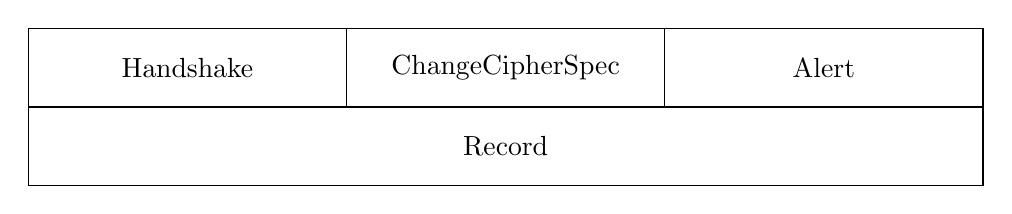
\begin{tikzpicture}
    \draw (0,0) rectangle (\textwidth, 1) node[pos=.5] {Record};
    \draw (0, 1) rectangle (\textwidth / 3,2) node[pos=.5] {Handshake};
    \draw (\textwidth / 3, 1) rectangle (\textwidth / 3 + \textwidth / 3, 2) node[pos=.5] {ChangeCipherSpec};
    \draw (\textwidth / 3 + \textwidth / 3, 1) rectangle (\textwidth / 3 + \textwidth / 3 + \textwidth / 3, 2) node[pos=.5] {Alert};
  \end{tikzpicture}

  \note{
    Von der Basis auf TCP kommt der Name Transport Layer Security.
    Record Protokoll: Arbeitet mit den eigentlichen Daten vom Application Layer, verschlüsselt diese, fragmentiert sie falls nötig und sendet sie zum Transport Layer, zusätzlich ist Kompression möglich.
    Alert Protokoll: Gibt Status an Gegenüber weiter: Fehler, Connectionabbrüche, etc.
    Handshake Protokoll: Kümmert sich um die Authentifizierung sowie Schlüsselaustausch und stellt eine Verbindung zwischen Client und Server her.
    ChangeCipherSpec Protokoll: Kann genutzt werden, um die Verschlüsslung zu wechseln.
  }
\end{frame}

\subsection{Motivation}

\begin{frame}{TLS 1.2}
Release: \textbf{vor 10 Jahren} \\
Letzte Änderungen dazu durch:
\begin{itemize}
    \item RFC6176, veröffentlicht in \textbf{\citeyear{RFC6176}}: \newline
    \textit{\citetitle{RFC6176}}
    \item RFC7627, veröffentlicht in \textbf{\citeyear{RFC7627}}: \newline
    \textit{\citetitle{RFC7627}}
    \item RFC7685, veröffentlicht in \textbf{\citeyear{RFC7685}}: \newline
    \textit{\citetitle{RFC7685}}
\end{itemize}
\end{frame}

\begin{frame}{Welche neuen, relevanten Technologien wurden entwickelt?}
  \begin{itemize}
    \item HTTP Public Key Pinning (HPKP) \autocite{RFC7469}
    \item Certificate Transparency (CT) \autocite{RFC6962}
    \item TLS False Start \autocite{RFC7918}
    \item Hash Key Derivation Function (HKDF) \autocite{RFC5869}
    \item Curve25519 sowie 448 \autocite{RFC7748}
    \item Edwards-curve Digital Signature Algorithm (EdDSA) \autocite{RFC8032}
    \item SHA3
  \end{itemize}

  \note{
    Disclaimer: Curve22519 is not a new technology.
    It was released in 2005.
    But after discovery that NSA implemented a backdoor into Dual\_EC\_DRBG, interest increased.
    Since 2017 NIST added them to Special Publication 800-186, allowing the use by US Federal Government.
  }
  \end{frame}

\begin{frame}{Welche Angriffe wurden seit TLS1.2 Release gefunden?}
  \begin{itemize}
    \item \textbf{Implementationsfehler}: Heartbleed, BERserk
    \item \textbf{\enquote{Downgrading}-Angriffe:} FREAK \& Logjam
    \item \textbf{\enquote{Cross-protocol}-Angriffe:} DROWN, Unholy PAC
    \item \textbf{\enquote{Chosen-plaintext}-Angriffe:} BEAST
    \item \textbf{Kompressions-basierte Angriffe:} CRIME, TIME, \& BREACH
    \item \textbf{\enquote{Padding oracle}-Angriffe:} POODLE, Serge Vaudenay's Angriff, Bleichenbacher's Oracle Angriff (ROBOT), Lucky13
    \item \textbf{Side-Channel-Angriffe:} HEIST
    \item \textbf{Angriffe auf spezifische Chiffre:} Sweet32, ROCA
    \item \textbf{Angriffe auf spezifische Hashing-Funktionen:} SLOTH
    \item \textbf{\enquote{Renegotiation}-Angriffe:} 3SHAKE
    \item \textbf{\enquote{Truncation}-Angriffe:} \citetitle{TruncatingTLS}
    \item \textbf{Resumption-basierte Angriffe:} \citetitle{TrackingUsers}
  \end{itemize}

  \note{
    RC4 Cipher attacks esp. bad in timing as it was recommended as mitigation against BEAST \\
    PKCS\#1 v1.5 sowie CBC ciphers ist oftmals Ursprung der Padding Oracle Angriffe.
    SHA1-Angriff SHAttered
  }
\end{frame}

\section{TLS 1.3}

\begin{frame}{TLS1.3}
  \begin{itemize}
    \item Release in August \citeyear{RFC8446}
    \item Spezifikation in RFC8446: \textit{\citetitle{RFC8446}}
    \item IETF began August 2013 mit ersten Arbeiten an TLS 1.3
    \item Erster Draft in April 2014 veröffentlicht wurden
    \item Unter anderem daran beteiligt:
    \begin{itemize}
      \item Google, Cloudflare, Akamai, Vodafone, Mozilla, Apple, Microsoft, Amazon, Facebook, Red Hat, IBM, ANSSI, Sun Microsystems, Nokia, Symantec, OpenSSL, Cisco...
    \end{itemize}
    \item Aufgrund signifikanter Änderungen beinahe TLS 2.0 oder gar 4.0 genannt\footnote{\url{https://www.ietf.org/mail-archive/web/tls/current/msg20938.html}}
  \end{itemize}

  \note{
    ANSSI = französischer Geheimdienst
  }
\end{frame}

\newcolumntype{Y}{>{\centering\arraybackslash}X}
\newcolumntype{S}{>{\centering\small}X}

\subsection{Browser- und Bibliotheksunterstützung}

\begin{frame}{Welche Browser unterstützen TLS 1.3?}
  \begin{tabularx}{\textwidth}{
      |>{\hsize=0.2\hsize} Y |
      >{\hsize=0.5\hsize} S |
      >{\hsize=0.2\hsize} Y |
      >{\hsize=0.1\hsize} Y |
    }
    \hline
    \textbf{Browser} & \textbf{Platforms} & \textbf{Versions} & \textbf{TLS 1.3}\\ \hline
    \multirow{2}{*}{Google Chrome}
        & \multirow{2}{*}{\parbox{6cm}{Windows (7+), Linux, Android (4.1+), Chrome OS, macOS (10.10+), iOS (9.0+)}}
          & 54 - 69 & \cellcolor{yellow!50}Disabled \\ \cline{3-4}
    & & 70 & \cellcolor{green!50}Yes \\ \hline
    \multirow{2}{*}[-0.75em]{Mozilla Firefox}
    & \multirow{2}{*}[-0.75em]{\parbox{6cm}{Windows (7+), Linux, Android (4.1+), macOS (10.9+), iOS (9.0+)}}
      & 49 - 62, ESR 52.0 - 60.3 & \cellcolor{yellow!50}Disabled \\ \cline{3-4}
    & & 63 & \cellcolor{green!50}Yes \\ \hline
    Internet Explorer & Windows (7+), Windows Server (2008 R2+) & IE 11 & \cellcolor{red!50}No \\ \hline
    \multirow{2}{*}{Microsoft Edge}
        & Windows 10 Mobile, Xbox & Edge 15 & \cellcolor{red!50}No \\ \cline{2-4}
    & Windows 10, Windows Server (2016+) & Edge 18 & \cellcolor{red!50}No \\ \hline
    Apple Safari & iOS 12, macOS 10.14 & 12 & \cellcolor{yellow!50}Disabled \\ \hline
    Opera Browser & Windows (7+), Linux, Android (4.0+), macOS (10.9+) & 56 & \cellcolor{yellow!50}Disabled \\ \hline
    Tor Browser & Windows (7+), Linux, macOS (10.9+) & IE 11 & \cellcolor{green!50}Yes \\ \hline
    \end{tabularx}

    \note{
      Chrome uses BoringSSL (Google's fork of OpenSSL) \\
      Firefox uses Mozilla's Network Security Services (NSS) \\
      Edge uses Microsoft's EdgeHTML on Windows, Apple/KDE's Webkit on iOS, and Chromium's Blink on Android \\
      Opera uses Apple/KDE's Webkit and Chromium's Blink \\
      Apple Safari apparently allows the use of TLS 1.3, but it is disabled and must be activated with \texttt{defaults write /Library/Preferences/com.apple.networkd tcp_connect_enable_tls13 1}\\
      Tor uses Firefox ESR 60.2 under the hood, which currently only implements the draft-22 version, but they are thinking about backporting NSS changes
    }
\end{frame}

\begin{frame}{Welche Bibliotheken unterstützen TLS 1.3?}
  \begin{tabularx}{\textwidth}{
    |>{\hsize=0.4\hsize} Y |
    >{\hsize=0.2\hsize} Y |
    >{\hsize=0.3\hsize} Y |
    >{\hsize=0.1\hsize} Y |
  }
  \hline
  \textbf{Library} & \textbf{Language} & \textbf{Versions} & \textbf{TLS 1.3}\\ \hline
  BoringSSL & C++ & \texttt{master} & \cellcolor{green!50}Yes \\ \hline
  fizz & C++ & v2018.11.12.00 & \cellcolor{green!50}Yes \\ \hline
  GnuTLS & C & 3.6.3 & \cellcolor{green!50}Yes \\ \hline
  Java Secure Socket Extension & Java & JDK11 & \cellcolor{green!50}Yes \\ \hline
  miTLS & F* & - & \cellcolor{green!50}Yes \\ \hline
  NSS & C / Assembler & 3.39 & \cellcolor{green!50}Yes \\ \hline
  OpenSSL & C & 1.1.1 & \cellcolor{green!50}Yes \\ \hline
  rustls & Rust & 0.14.0 & \cellcolor{green!50}Yes \\ \hline
  SChannel (Windows API) & C++ & Windows 10 v1607 & \cellcolor{red!50}No \\ \hline
  Secure Transport & C / Swift & macOS 10.13, iOS 11 & \cellcolor{yellow!50}Yes \\ \hline
  wolfSSL & C & 3.15 & \cellcolor{green!50}Yes \\ \hline
  \end{tabularx}

  \note{
    cryptlib is a library from Peter Gutmann, a Professor in Auckland \\
    JSSE (Java) will need JDK11, but other library like Bouncy Castle is good too. \\
  }
\end{frame}

\subsection{Allgemeine Änderungen}

\begin{frame}{Allgemeine Änderungen}
  \begin{itemize}
    \item ChangeCipherSpec wurde entfernt, somit bleibt über: \\
    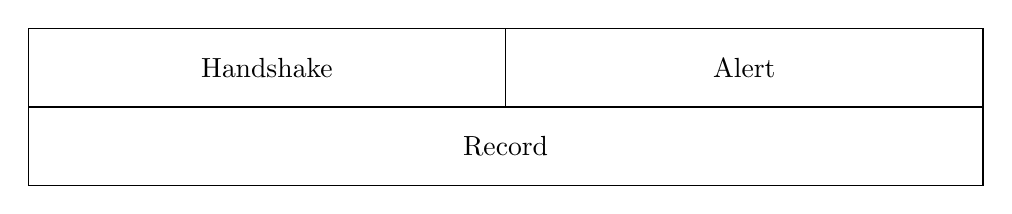
\begin{tikzpicture}
      \draw (0,0) rectangle (\textwidth, 1) node[pos=.5] {Record};
      \draw (0, 1) rectangle (\textwidth / 2,2) node[pos=.5] {Handshake};
      \draw (\textwidth / 2 , 1) rectangle (\textwidth / 2 + \textwidth / 2, 2) node[pos=.5] {Alert};
    \end{tikzpicture}
    \item Renegotiation zu SSL untersagt
    \item Nutzer-definierte Diffie-Hellmann Gruppen nicht mehr unterstützt
    \item Nur noch Schlüsselaustauschprotokolle, die Perfect Forward Secrecy garantieren:
    \begin{itemize}
      \item DHE-RSA,
      \item ECDHE-RSA,
      \item ECDHE-ECDSA
    \end{itemize}
  \end{itemize}

  \note{
    Entfernen der Custom DHE Groups macht es erst möglich, dass ein ganzer Round Time Trip vom Handshake entfernt werden kann, da der Client einfach welche zu Beginn des Verbindungsaufbaus auswählt und daher nicht erst mit dem Server aushandeln muss, welche benutzt werden müssen
    Erlaubt sind also nur noch die Schlüsselaustauschprotokolle, die auf ephemeral Diffie-Hellmann (über finite Felder oder elliptic-curve) oder auf einem pre-shared Key aufbauen.
    Das bedeutet, dass statisches RSA oder DSA gar nicht mehr erlaubt ist.
  }
\end{frame}

\subsection{Änderungen am Handshake-Protokoll}

\begin{frame}{TLS v1.2 Handshake}
  \begin{figure}[!h]
    \centering
    \vspace*{-0.5cm}
    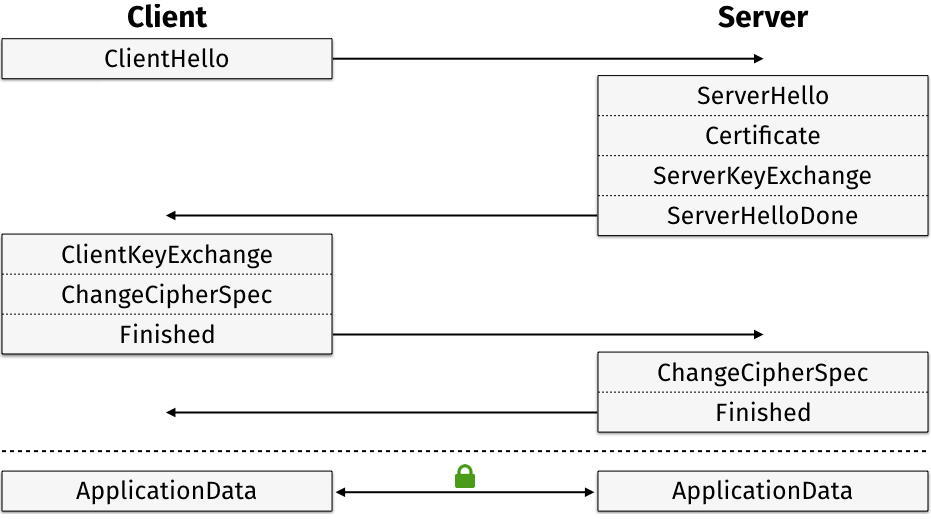
\includegraphics[scale=0.375,keepaspectratio]{./images/tls12-handshake-ecdhe.png}
    %\caption{TLS 1.2 Handshake mit ECDHE}
    \label{fig:tls12-handshake-ecdhe}
    \autocite{taubert}
  \end{figure}

  \note{
    ECDHE daher, weil static RSA ab TLS 1.3 nicht mehr unterstützt ist.
    Bei static RSA würde ServerKeyExchange nicht durchgeführt werden.
    Base Key zum Verschlüsseln ab EncryptedExtensions hier ist das \texttt{server_handshake_traffic_secret}
  }
\end{frame}

\begin{frame}{TLS v1.3 Handshake}
  \begin{figure}[!h]
    \centering
    \vspace*{-0.25cm}
    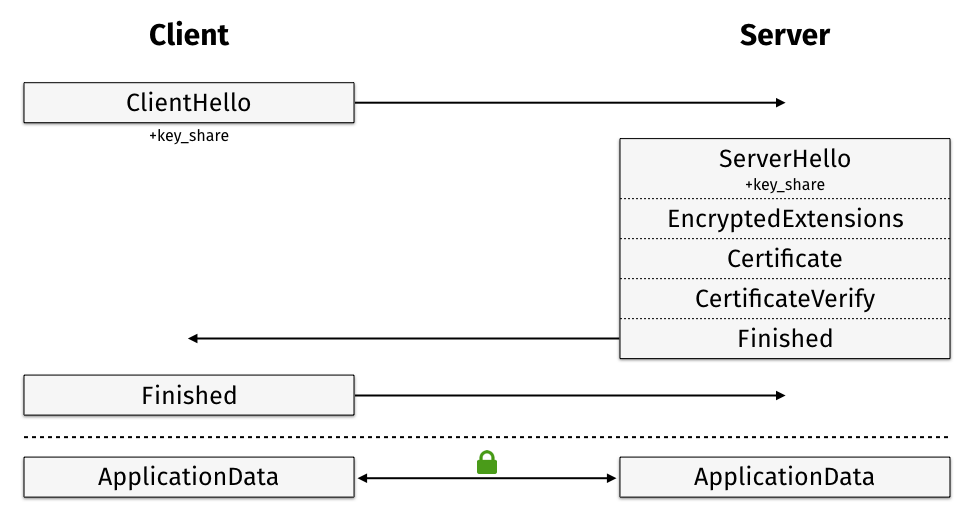
\includegraphics[width=\linewidth]{./images/tls13-handshake-ecdhe.png}
    %\caption{TLS 1.3 Handshake mit ECDHE}
    \label{fig:tls13-handshake-ecdhe}
  \end{figure}

  \note{
    Möglich, da RSA und Custom DH Groups entfernt wurden.
    Durch festgesetzte finite Gruppen für den Diffie-Hellmann Austausch ist es einfach zu entscheiden, welche Parameter wohl vom Server unterstützt werden (entweder ECDHE mit x25519, P-256).
    Dadurch kann Client KeyShares direkt mitschicken, es verfällt das Bedürfnis darüber zu verhandeln und wir sparen uns einen RoundTrip
  }
\end{frame}

\begin{frame}{0-RTT Handshake}
  \begin{figure}[!h]
    \centering
    \vspace*{-0.25cm}
    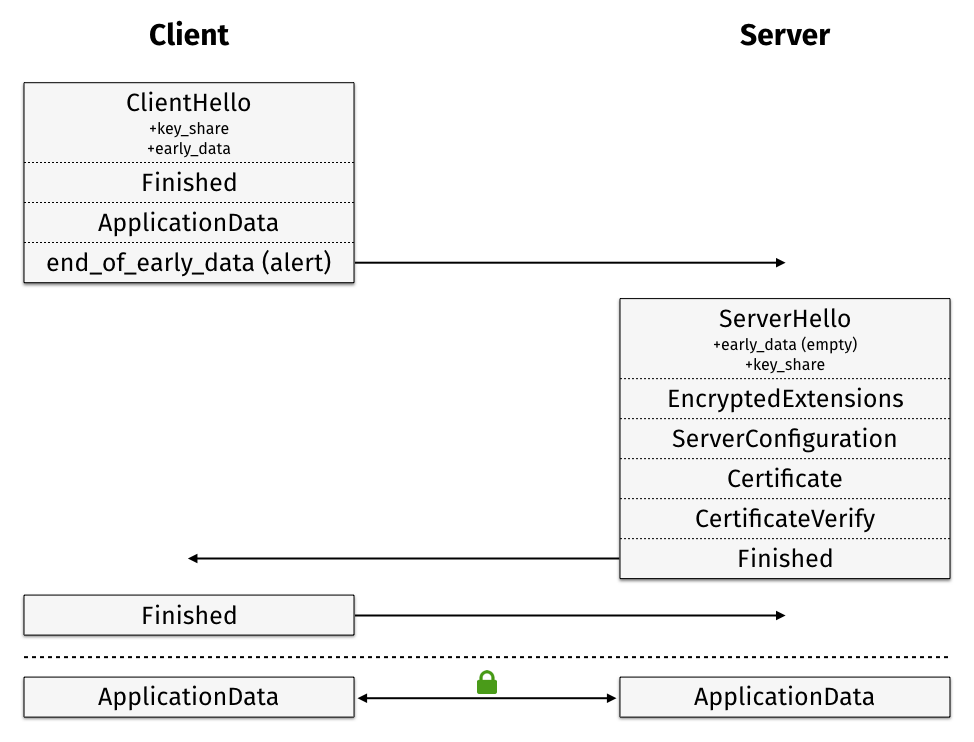
\includegraphics[width=\linewidth]{./images/tls13-handshake-zero-rtt.png}
    %\caption{TLS 1.3 Handshake mit ECDHE}
    \label{fig:tls13-handshake-zero-rtt}
  \end{figure}
  \note{
    0-RTT sind anfällig gegenüber Replayattacken
    Müssen daher idempotent sein, wird geraten nur bei GET zu erlauben
    Anwesenden fragen, ob sie eventuell Problem mit dem 0-RTT Handshake sehen
  }
\end{frame}

% \subsection{Session Resumption}

% \begin{frame}{Session Resumption basierend auf einem \enquote{pre-shared key}-Modus}
%   \begin{figure}[!h]
%     \centering
%     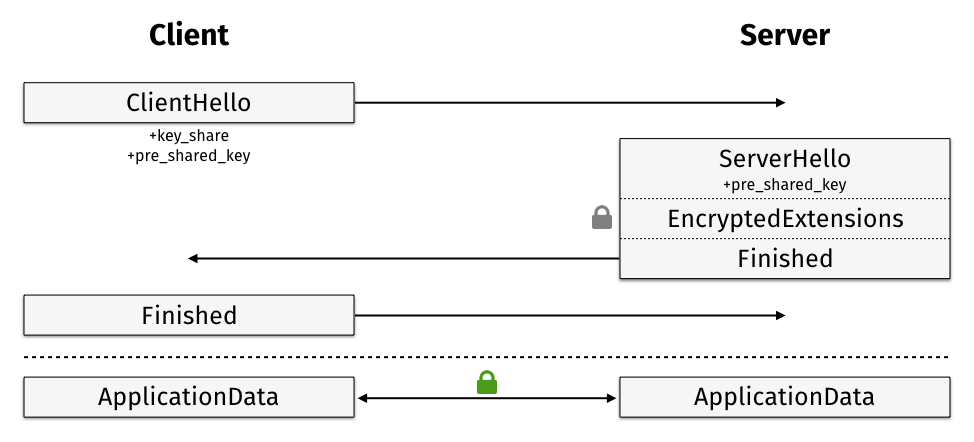
\includegraphics[width=\linewidth]{./images/tls13-handshake-resumption.png}
%     %\caption{TLS 1.3 Handshake mit ECDHE}
%     \label{fig:tls13-handshake-resumption}
%     \autocite{taubert}
%   \end{figure}
% \end{frame}

\begin{frame}{Was ist \enquote{downgrading}?}
\begin{itemize}
  \item Herabstufung von Protokollparametern zu gefährlichen Werten:
  \begin{itemize}
    \item Von TLS 1.2 auf SSL 2.0
    \item Von DHE (1024-Bit Schlüssel und aufwärts) auf DHE_EXPORT (maximal 512-Bit)
  \end{itemize}
  \item Angreifer zwingt Client und Server zu schwächeren Sicherheitsmaßnahmen
  \item Beispielsweise Ändern der Supported Cipher Suite Liste durch Man-in-the-Middle-Angriff
  \item Bisher bekannte Angriffe dieser Art: FREAK und LogJam
\end{itemize}
\end{frame}

\begin{frame}{LogJam-Angriff: Theorie}
  \begin{figure}[!h]
    \centering
    \vspace*{-0.35cm}
    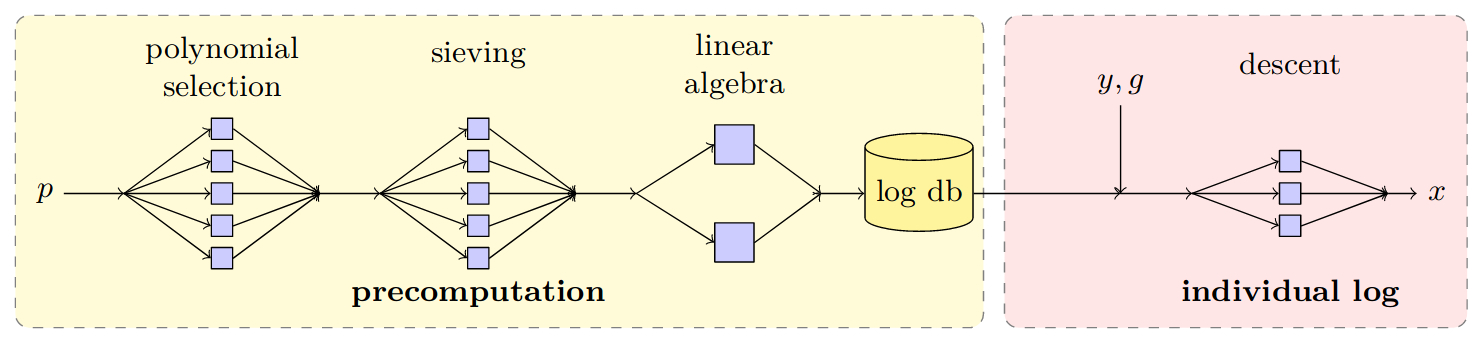
\includegraphics[width=\linewidth]{./images/logjam-discrete-log-problem.jpg}
    \caption{Der Zahlkörpersieb-Algorithmus für diskreten Logarithmus}
    \label{fig:logjam-theory}
  \end{figure}
  \begin{itemize}
    \item Diskreter Logarithmus bestmöglichst kryptoanalytische Angriffsmethode beim Diffie-Hellman
    \item Angreifer muss nur $log(x)$ für $y = (g^x) mod p$ berechnen
    \item Danach hat er das shared secret
  \end{itemize}

  \note {
    Essentiell wird im Precomputation-Schritt eine Matrix aufgebaut, die Log DB, die die Prime-Factorizationen enthält, die gefunden wurden für ein bestimmtes P / eine bestimmte Primzahl. Einmal berechnet, kann der vorberechnete Schritt immer wieder für dieses bestimmte P genutzt werden.

    Wichtig ist, dass das alles vorberechnet werden kann.
    Nur der Descent-Schritt muss zur Laufzeit verarbeitet werden.
    Hier wird y wieder faktorisiert und durch ein Sieb gelaufen, bis es möglich ist, diese faktorisierten Primzahlen durch vorhandene Elemente in der Log-DB nachzustellen.
  }
\end{frame}

\begin{frame}{LogJam-Angriff: Ablauf}
  \begin{figure}[!h]
    \centering
    \vspace*{-0.35cm}
    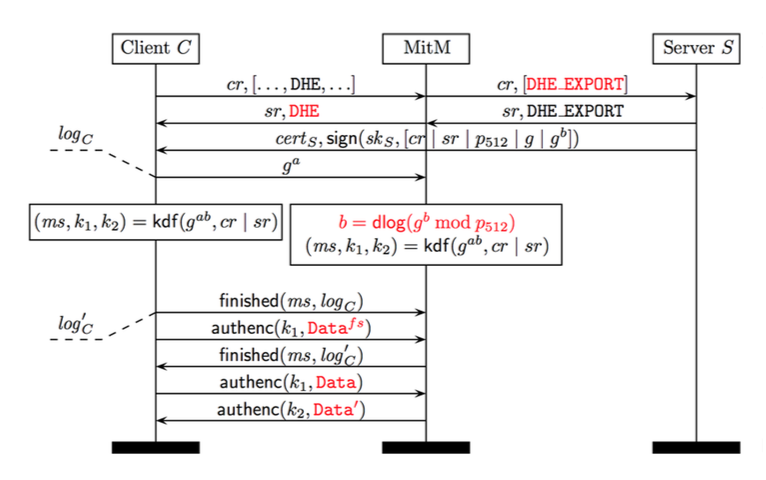
\includegraphics[scale=0.8]{./images/logjam.png}
    %\caption{TLS 1.3 Handshake mit ECDHE}
    \label{fig:logjam-runthrough}
    \autocite{logjam}
  \end{figure}

  \note {
    Die Eleganz des Angriffs liegt dadrinne, dass ein MitM zur Laufzeit den Verbindungsaufbau des Clients C abfängt und die gewünschte Cipher Suite auf DHE_EXPORT setzt, dessen Primezahlen nicht mehr als 512-Bit haben dürfen.
    Der Designfehler hier in TLS ist folgender: die ServerKeyExchange Antwort des Servers, hier cert_S ähnelt dem Aufbau für normale DHE Cipher Suites und macht keine Aussage darüber, welche Cipher Suite vom Server gewählt wurde. Dadurch kann der Client nicht bemerken, dass hier auf DHE_EXPORT gewechselt wurde.
  }
\end{frame}

\begin{frame}{LogJam-Angriff: Wie praktikabel ist dieser Angriff?}
  \begin{figure}[!h]
    \centering
    \vspace*{-0.35cm}
    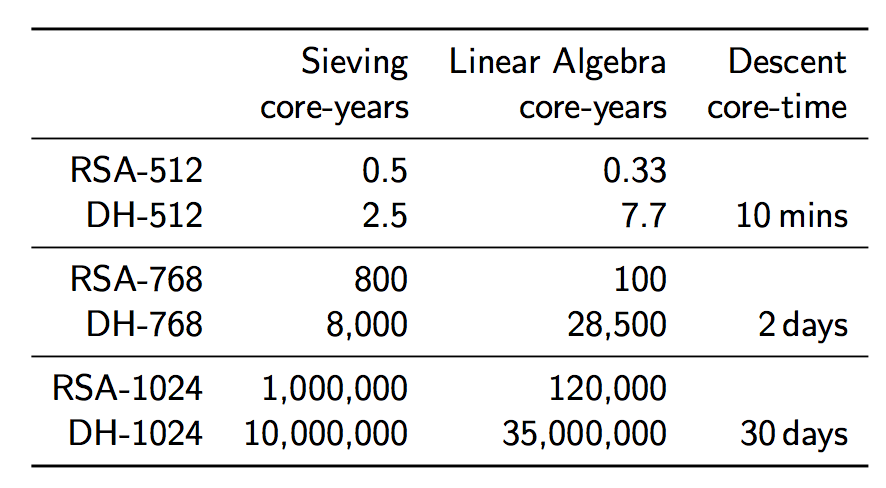
\includegraphics[scale=0.55]{./images/logjam-speeds.png}
    %\caption{TLS 1.3 Handshake mit ECDHE}
    \label{fig:logjam-practical}
  \end{figure}

  \begin{itemize}
    \item Geschwindigkeitsschub durch ASICs und Supercomputer
    \item Laut Paper nur 1 Jahr für Sieb sowie Linear Algebra Schritt bei DH-1024 dadurch
    \item Kostet \enquote{nur} 130 Millionen US-Dollar...
    \item ... nur 1\% des 2012 Budget der NSA :(
  \end{itemize}
\end{frame}

\begin{frame}{Downgrading Präventions-Mechanismus in TLS 1.3}
Direkte Fixes gegen LogJam:
\begin{itemize}
  \item Export Cipher Suites sind nicht mehr erlaubt
  \item Nutzer-definierte Diffie-Hellman Gruppen auch nicht erlaubt
  \item Wechsel zu Kryptografie basierend auf Elliptischen Kurven
\end{itemize}
Weitere Fixes gegen generelle Downgrading-Angriffe:
\begin{itemize}
  \item Server signiert den gesamten Handshake, inkl. Cipher Negotiation
  \item Dadurch kann kein Downgrading mehr passieren
\end{itemize}

\note{
  Für TLS 1.2 sieht das hier anders aus:
  Web Server muss entsprechend konfiguriert werden. Darf keine Nutzer-definierten Gruppen zulassen, keine DHE_EXPORT Cipher Suites.
  Muss idealerweise mindestens 2048-bit Keys zulassen.
}
\end{frame}

\subsection{Entfernte Funktionalität}

\begin{frame}{Warum sollte man Funktionalität entfernen?}
  \begin{overlayarea}{\textwidth}{.5\textheight}
  \begin{itemize}
    \item<2-> Neu gefundene Attacken schwächen vorhandene Funktionalität
    \item<3-> Funktionalität sicherheitstechnisch nicht abgesichert
    \item<4-> Protokoll zu flexibel, richtige Konfiguration muss gewählt werden
    \end{itemize}
  \end{overlayarea}

    \note{
      Anwesenden fragen, ob sie gute Ideen hätten, warum man Funktionalität entfernt.
    }
\end{frame}

\begin{frame}{Cipher Suite Änderungen}
  \begin{itemize}
  \item HKDF wird als Grundlage aller Schlüsselaustauschprotokolle genutzt
  \item Stromchiffre ChaCha20 mit MAC Poly1305 hinzugefügt
  \item Digitale Signature Algorithmen Ed25519 und Ed448 hinzugefügt
  \item Schlüsselaustauschprotokolle Curve25519 und Curve448 hinzugefügt
  \item RC4, SHA1 und MD5 Support entfernt \autocite{rc4.nomore} \autocite{shattered}
  \item RSASSA-PSS statt RSA PKCS\#1v1.5
  \item CBC MAC-then-Encrypt Modes nicht mehr unterstützt
\end{itemize}
\note {
  Cipher Suite = Chiffrensammlung
  Definiert Schlüsselaustauschprotokoll (RSA, ECDHE), Authentifizierungsalgorithmus (RSA, DSA, ECDSA),
  Verschlüsslungalgorithmus (RC4, Triple DES, AES) und Hashfunktion (SHA1, SHA256), MAC-Funktion (HMAC mit SHA1...)
  TLS_RSA_WITH_3DES_EDE_CBC_SHA

  Als Stromchiffre ist nur eben genannte erlaubt,
  Als Blockchiffre nur AES GCM / CCM.
}
\end{frame}

\begin{frame}{Erlaubte Cipher Suites}
Nur noch Authenticated Encryption with Associated Data (AEAD) basierte Cipher Suites erlaubt
Nomenklatur: TLS\_AEAD\_HASH
  \begin{itemize}
    \item TLS\_AES\_128\_GCM\_SHA256
    \item TLS\_AES\_256\_GCM\_SHA384
    \item TLS\_CHACHA20\_POLY1305\_SHA256
    \item TLS\_AES\_128\_CCM\_SHA256
    \item TLS\_AES\_128\_CCM\_8\_SHA256
  \end{itemize}

\begin{itemize}
  \item Dadurch werden folgende Attacken vermieden:
  \begin{itemize}
    \item Vaudenay, Lucky13, LuckyMinus20, POODLE, Bleichenbacher (ROBOT)
  \end{itemize}
\end{itemize}
\end{frame}

\begin{frame}{Lucky13-Angriff}
\end{frame}

\begin{frame}{Kompression}
\begin{itemize}
  \item TLS 1.2 erlaubt optionale Kompression
  \item Definiert in RFC3749: \citetitle{RFC3749}
  \item Gesamter Datentransfer wird komprimiert, inkl. HTTP Header
  \item Erlaubte Methoden: DEFLATE, LZS
  \item Unterstützung für Kompression in TLS 1.3 \textbf{komplett} entfernt
\end{itemize}
\end{frame}

\begin{frame}[fragile]{CRIME-Angriff}
\begin{itemize}
  \item Basiert auf Kompressionsmethode DEFLATE
  \item DEFLATE ersetzt zweite Instanz einer Bytesequenz durch kleines Token
  \item Token besagt: An dieser Stelle, selbe Sequenz wie n Bytes zuvor mit Length x
  \item Angreifer kennt Cookienamen
\end{itemize}
\begin{lstlisting}[frame=single]
POST / HTTP/1.1
Host: thebankserver.com
Cookie: secret=7xc89f94wa
... // Body beginnt
Cookie: secret=0
\end{lstlisting}
\note {
  Pakete mit secret = 0 bis 6 haben die selbe Länge
  Paket mit secret=7 ist eins kürzer, da DEFLATE besser komprimieren kann
  Angreifer kann Secret Byte für Byte rekonstruieren
}
\end{frame}

\begin{frame}{Renegotiation}
3SHAKE Angriff
\end{frame}

\section{Fazit}

\begin{frame}{Welche Angriffe wurden durch TLS 1.3 verhindert?}

  \begin{tabularx}{\textwidth}{
    |>{\hsize=0.3\hsize} Y |
    >{\hsize=0.4\hsize} Y |
    >{\hsize=0.3\hsize} Y |
  }
  \hline
  \textbf{Angriffstyp} & \textbf{Bekannte Angriffe} & \textbf{Mitigation in TLS 1.3}\\ \hline
  Implementationsfehler & Heartbleed, BERserk & Nicht verhinderbar \\ \hline
  Downgrading & FREAK, LogJam & Protokoll-Downgrade nicht erlaubt, Export Cipher entfernt \\ \hline
  Cross-protocol & DROWN, Unholy PAC & Protokoll-Downgrade nicht erlaubt \\ \hline
  Chosen-plaintext & BEAST & CBC Cipher Suites entfernt \\ \hline
  Kompressions-basiert & CRIME, TIME, BREACH & TLS-Kompression entfernt \\ \hline
  Padding oracle & POODLE, Vaudenay's Angriff, Bleichenbacher's Angriff, Lucky13 & RSA-PKCS\#1 v1.5, CBC Cipher Suites entfernt, nur AEAD Cipher \\ \hline
  \end{tabularx}


  \note{
  }
\end{frame}

\begin{frame}{Welche Angriffe wurden durch TLS 1.3 verhindert?}
  \begin{tabularx}{\textwidth}{
    |>{\hsize=0.3\hsize} Y |
    >{\hsize=0.4\hsize} Y |
    >{\hsize=0.3\hsize} Y |
  }
  \hline
  \textbf{Angriffstyp} & \textbf{Bekannte Angriffe} & \textbf{Mitigation in TLS 1.3}\\ \hline
  Side-Channel & HEIST & - \\ \hline
  Chiffre-basiert & Sweet32, ROCA & Schwache (3DES bspw.) Cipher Suites entfernt \\ \hline
  Hashing-Funktion-basiert & SLOTH & MD5, SHA1 nicht erlaubt \\ \hline
  Renegotiation & 3SHAKE & Renegotiation nicht erlaubt \\ \hline
  Truncation & \autocite{TruncatingTLS} & - \\ \hline
  Resumption-basiert & \autocite{TrackingUsers} & Session Resumption deaktivieren \\ \hline
  \end{tabularx}

  \note{
  }
\end{frame}

\begin{frame}{Fazit}
\begin{itemize}
  \item Flexibilität schwindet...
  \item .. dafür Konfigurationsaufwand geringer
  \begin{itemize}
    \item Schwerer, eine unsichere Konfiguration zu konzipieren
  \end{itemize}
  \item Gefährliche Features verschwunden
  \item Viele Sicherheitslücken im Keim erstickt
\end{itemize}
\end{frame}

\begin{frame}[standout]
  Offene Fragen?
\end{frame}

\section{Literatur}

\begin{frame}[allowframebreaks]{Literatur}
  \printbibliography
\end{frame}

\end{document}
